\documentclass{article}
\usepackage{graphicx}
\usepackage{adjustbox,lipsum}
\begin{document}

\title{Networks \& Security Lab}
\author{}
\date{}
\maketitle

\begin{abstract}
This document presents the tasks and activities held in Network Security Lab in the first lab class. The problems were based on the basic ciphers in \textbf{Cryptography}.
\end{abstract}

\section{Topic}
	\subsection{Extended Euclidean Algorithm}
	
	\begin{figure}
	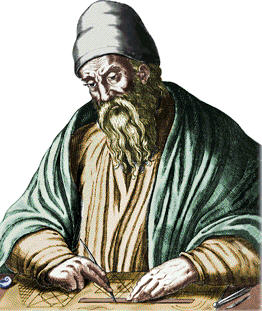
\includegraphics[width=\linewidth]{Euklid_von_Alexandria_1.jpg}
	\caption{Euclid}
	\label{fig : Euclid}
	\end{figure}
	
Figure \ref{fig : Euclid} shows Euclid	
		\textbf{Problem Statement} \\
			Given the two numbers $a$ and $b$, find the two numbers $x$ and $y$ such that they satisfies the equation 
			\begin{equation}
    				a x + b y = \gcd(a,b)
			\end{equation}
			
		\textbf{Input} \\
				A line containing two integers $a$ and $b$ \\

		\textbf{Output} \\
				A line containing two integers $x$ and $y$ \\

		
			\textbf{Constrains} \\
			
				$1 \leq a,b \leq 10^{6}$\\


		
			\textbf{Memory Limit}
				$256 MB$
	
		 	\textbf{Time Limit}
				$1 \, sec$ for each test case file

	\subsection{Vigenère Cipher}
	
		\textbf{Problem Statement} \\
			Given an upper-case alphabetic string Plain-text p and a upper-case alphabetic string keyword  key, your task is to \\
		\begin{itemize}
			\item  Encrypt the plain-text using key and give the output as cipher-text cipher.
			\item  Decrypt the cipher-text cipher obtained above to get the original plain-text.
		\end{itemize}			


\begin{table}[ht]
\centering
\caption{Table To Encrypt}
\begin{adjustbox}{width=1\textwidth}
\small
\begin{tabular}{|l|llllllllllllllllllllllllll|} 
\hline
  & A & B & C & D                      & E & F & G & H & I & J & K & L & M & N & O & P & Q & R & S & T & U & V & W & X & Y & Z  \\ 
\hline
A & A & B & C & D                      & E & F & G & H & I & J & K & L & M & N & O & P & Q & R & S & T & U & V & W & X & Y & Z  \\
B & B & C & D & E                      & F & G & H & I & J & K & L & M & N & O & P & Q & R & S & T & U & V & W & X & Y & Z & A  \\
C & C & D & E & F                      & G & H & I & J & K & L & M & N & O & P & Q & R & S & T & U & V & W & X & Y & Z & A & B  \\
D & D & E & F & G                      & H & I & J & K & L & M & N & O & P & Q & R & S & T & U & V & W & X & Y & Z & A & B & C  \\
E & E & F & G & H                      & I & J & K & L & M & N & O & P & Q & R & S & T & U & V & W & X & Y & Z & A & B & C & D  \\
F & F & G & H & \multicolumn{1}{l|}{I} & J & K & L & M & N & O & P & Q & R & S & T & U & V & W & X & Y & Z & A & B & C & D & E  \\
G & G & H & I & J                      & K & L & M & N & O & P & Q & R & S & T & U & V & W & X & Y & Z & A & B & C & D & E & F  \\
H & H & I & J & K                      & L & M & N & O & P & Q & R & S & T & U & V & W & X & Y & Z & A & B & C & D & E & F & G  \\
I & I & J & K & L                      & M & N & O & P & Q & R & S & T & U & V & W & X & Y & Z & A & B & C & D & E & F & G & H  \\
J & J & K & L & M                      & N & O & P & Q & R & S & T & U & V & W & X & Y & Z & A & B & C & D & E & F & G & H & I  \\
K & K & L & M & N                      & O & P & Q & R & S & T & U & V & W & X & Y & Z & A & B & C & D & E & F & G & H & I & J  \\
L & L & M & N & O                      & P & Q & R & S & T & U & V & W & X & Y & Z & A & B & C & D & E & F & G & H & I & J & K  \\
M & M & N & O & P                      & Q & R & S & T & U & V & W & X & Y & Z & A & B & C & D & E & F & G & H & I & J & K & L  \\
O & O & P & Q & R                      & S & T & U & V & W & X & Y & Z & A & B & C & D & E & F & G & H & I & J & K & L & M & N  \\
P & P & Q & R & S                      & T & U & V & W & X & Y & Z & A & B & C & D & E & F & G & H & I & J & K & L & M & N & O  \\
Q & Q & R & S & T                      & U & V & W & X & Y & Z & A & B & C & D & E & F & G & H & I & J & K & L & M & N & O & P  \\
R & R & S & T & U                      & V & W & X & Y & Z & A & B & C & D & E & F & G & H & I & J & K & L & M & N & O & P & Q  \\
S & S & T & U & V                      & W & X & Y & Z & A & B & C & D & E & F & G & H & I & J & K & L & M & N & O & P & Q & R  \\
T & T & U & V & W                      & X & Y & Z & A & B & C & D & E & F & G & H & I & J & K & L & M & N & O & P & Q & R & S  \\
U & U & V & W & X                      & Y & Z & A & B & C & D & E & F & G & H & I & J & K & L & M & N & O & P & Q & R & S & T  \\
V & V & W & X & Y                      & Z & A & B & C & D & E & F & G & H & I & J & K & L & M & N & O & P & Q & R & S & T & U  \\
W & W & X & Y & Z                      & A & B & C & D & E & F & G & H & I & J & K & L & M & N & O & P & Q & R & S & T & U & V  \\
X & X & Y & Z & A                      & B & C & D & E & F & G & H & I & J & K & L & M & N & O & P & Q & R & S & T & U & V & W  \\
Y & Y & Z & A & B                      & C & D & E & F & G & H & I & J & K & L & M & N & O & P & Q & R & S & T & U & V & W & X  \\
Z & Z & A & B & C                      & D & E & F & G & H & I & J & K & L & M & N & O & P & Q & R & S & T & U & V & W & X & Y  \\
\hline
\end{tabular}
\end{adjustbox}
\end{table}

			
		\textbf{Input} \\
				Two strings \\
				\begin{itemize}
			\item  Plaintext 
			\item  Key
		\end{itemize}	
		\textbf{Output} \\
				\begin{itemize}
			\item Cipher-text
			\item  Plain-text
		\end{itemize}	
		
			\textbf{Constrains} \\
			
				Strings length $\leq 10^6$


		
			\textbf{Memory Limit}
				$256 MB$
	
		 	\textbf{Time Limit}
				$1 \, sec$ for each test case file

\section{Expectation From Students}
		The student should be able to convert the theory of Euclid Algorithm into the program. He/ She should be able to write the code in C Language keeping in mind the constrains.\\ \\

		The student should be able to formulate the ciphers and using alpha-numeric conversion with addition to some modulo property would implement the algorithm correctly. \\ \\
 The code should be syntactically correct, efficient as well as logically correct. To ensure the correctness of program the student has to design his own test cases and check them manually. The test cases against which the code output would be tested is being hidden from the student. The student should ask any doubt regarding the problem or the online judge platform on \textbf{piazza platform}.
	\section{Evaluation}
		The evaluation of the lab assignment is done by \textbf{Online Judge - Hackerearth}. The code has to be made on online text editor where the student is under continuous surveillance by web cam. The student have to make solution in stipulate and submit it on the online judge. Then the program is being checked for any compilation error. If there are no compilation error then the program is measured against various parameters for grading which includes \\
\begin{itemize}
	\item Efficiency in both Time \& Space Complexity
	\item Comparing the output of student program and correct output which is already precomputed but hidden
\end{itemize}

Moreover, the online judge is full screen with copy/paste disable outside the text editor. There are 5 test case file at the back-end which are hidden from the student and the student's code is run against these test case files. If all the outputs of a test case file's outputs matches the student's output then 20 \% marks has been graded to the student. Otherwise no marks for that test case file. 
		
\section{Outcome}
After the succesful completion of assignment the student would be able to understand \\ The Euclid extended algorithm which plays a major role in the almost all the algorithms of the cryptography which involves numbers as gcd defines whether two numbers are co prime or not.The extended Euclidean algorithm is particularly useful when a and b are co-prime (or gcd is 1). Since x is the modular multiplicative inverse of “a modulo b”, and y is the modular multiplicative inverse of “b modulo a”. In particular, the computation of the modular multiplicative inverse is an essential step in RSA public-key encryption method.\\

The students will get to know about the \textbf{poly-alphabetic substitution} cipher which involves the extended use of Caesar ciphers. Since this cipher uses the modulo properties then this will be useful in disguising the plain-text letter frequency to interfere with a straightforward application of frequency analysis. 
\end{document}
